\section{Model 3}


The results displayed in this section are for the uncertainty involved in the calculation of flamespeed depending  on two parameter i.e the activation energy for the fall off reaction in the ozone mechanism and the pre exponential factor for third reaction in the mechanism. The percentage of ozone is taken as 40, 46, 53, 75, and 100  percent according to the experimental data available to us from Streng\cite{Streng}. In the
figure~\ref{subfig-4:KDE for $A_3$} and figure~\ref{subfig-4:KDE2 for $E_3$},  we display results for sample size 1e7 and surrogate
of 100X100 points.  We show the the KDE for parameters log($A_3$) and $E_3$.

\bigskip

In the figure~\ref{subfig-4:samp for $A_3$} and figure~\ref{subfig-4:samp for $E_3$} , for
constant surrogate size of 100x100, the number of samples are changed from 1e5 to
1e7 and convergence is observed. The plot is done for raw chain size of $1e7$, $2e7$ , $5e7$, and $9e7$ is taken. In the figure~\ref{subfig-5:surr for $A_3$} and figure~\ref{subfig-5:surr2 for $E_3$},
convergence study is done for surrogates with differing number of interpolation points. As we increase the number of points in the surrogate, results should be close for different surrogate sizes. The plot is done for surrogate size of 75X75, 100X100 150X150 , and 200X200 for both parameters log($A_3$) and $E_3$. In this analysis, raw sample chain size is $1e7$. For different starting points of MCMC chain, the MAP point of the resulting pdf does not change. The surrogates for individual concentrations are constructed using linear interpolation
function. The initial guess for the MAP point is calculated using Nelder Mead optimization technique. 

\bigskip

In the
figure~\ref{subfig-1:mean_3} and figure~\ref{subfig-2:autocr_3},  mean and correlation plots are shown for
the samples of the parameters log($A_3$) and $E_3$. The mean plot shows the initial instability due to sum in period of MCMC and after that it remains constant. It shows us that we should be using at least more than these number of samples for our analysis. The figure~\ref{subfig-1:a3_distribution} shows the posterior of the parameter log($A_3$) with the following parameters of the distribution-Mean:  32.86, Std. Dev.:  0.97, Skewness:  -0.96, and Kurtosis:  1.79.  The figure~\ref{subfig-1:e3_distribution_3} shows the posterior of the parameter $E_3$ with the following parameters of the distribution- Mean:  57.50, Std. Dev.:  8.36, Skewness:  -0.77, and Kurtosis:  1.20.


\bigskip

 It is necessary to ensure that the samples of the parameter which we are drawing are fitting the flamespeed values of the experiment. In the figure~\ref{subfig-1:40_3}, figure~\ref{subfig-2:46_3}, figure~\ref{subfig-3:53_3}, figure~\ref{subfig-4:75_3}, and figure~\ref{subfig-5:100_3},   we calculate the flamespeed for all the parameters drawn using the surrogate generated before for 40$\%$, 46$\%$, 53$\%$, 75$\%$, and 100 $\%$ respectively. We have taken $1e7$ sample size and calculated flamespeed for all the concentrations of ozone mentioned. We have a good fit to the data overall.




\begin{figure}[H]
\subfloat[KDE \label{subfig-4:KDE for $A_3$}]{
        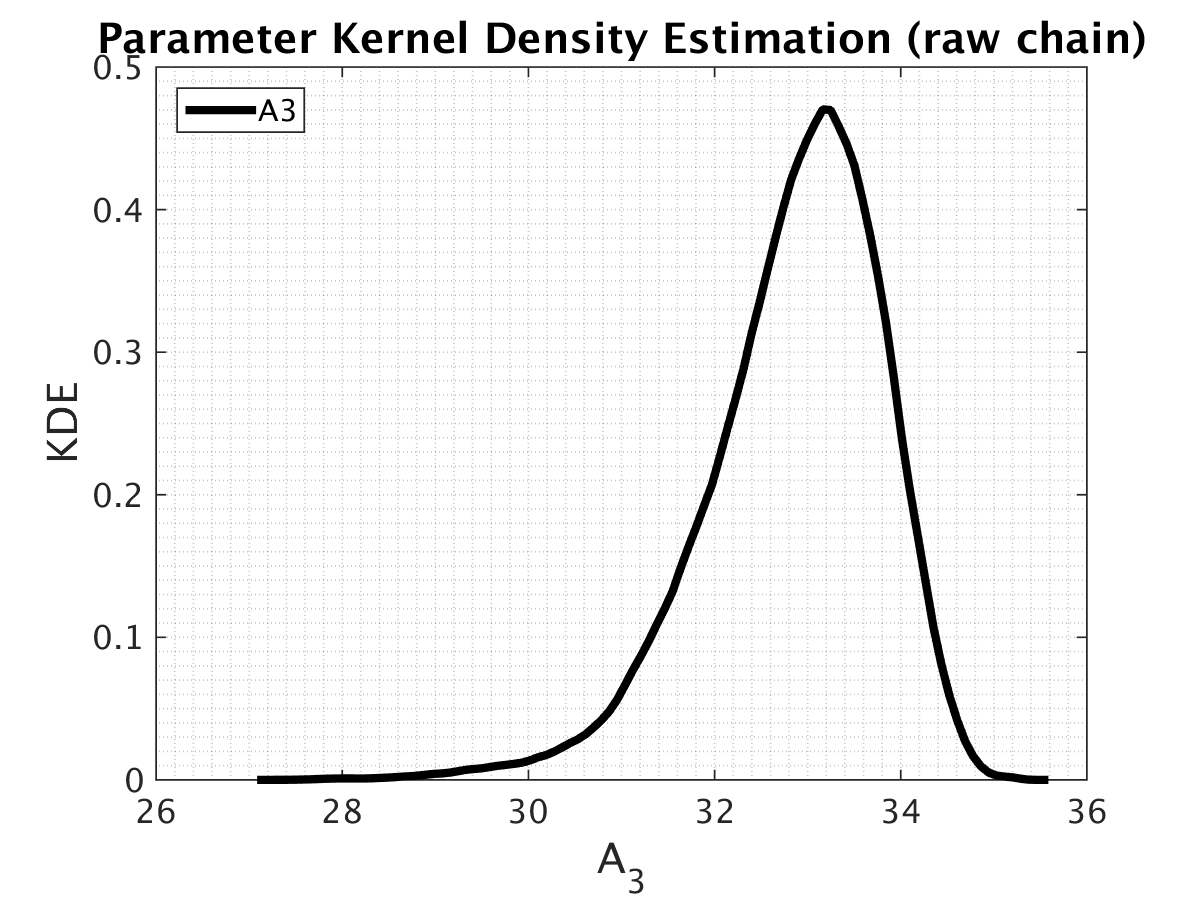
\includegraphics[scale=0.45]{model_3/kde_1} 
            }             
\subfloat[KDE \label{subfig-4:KDE2 for $E_3$}]{
        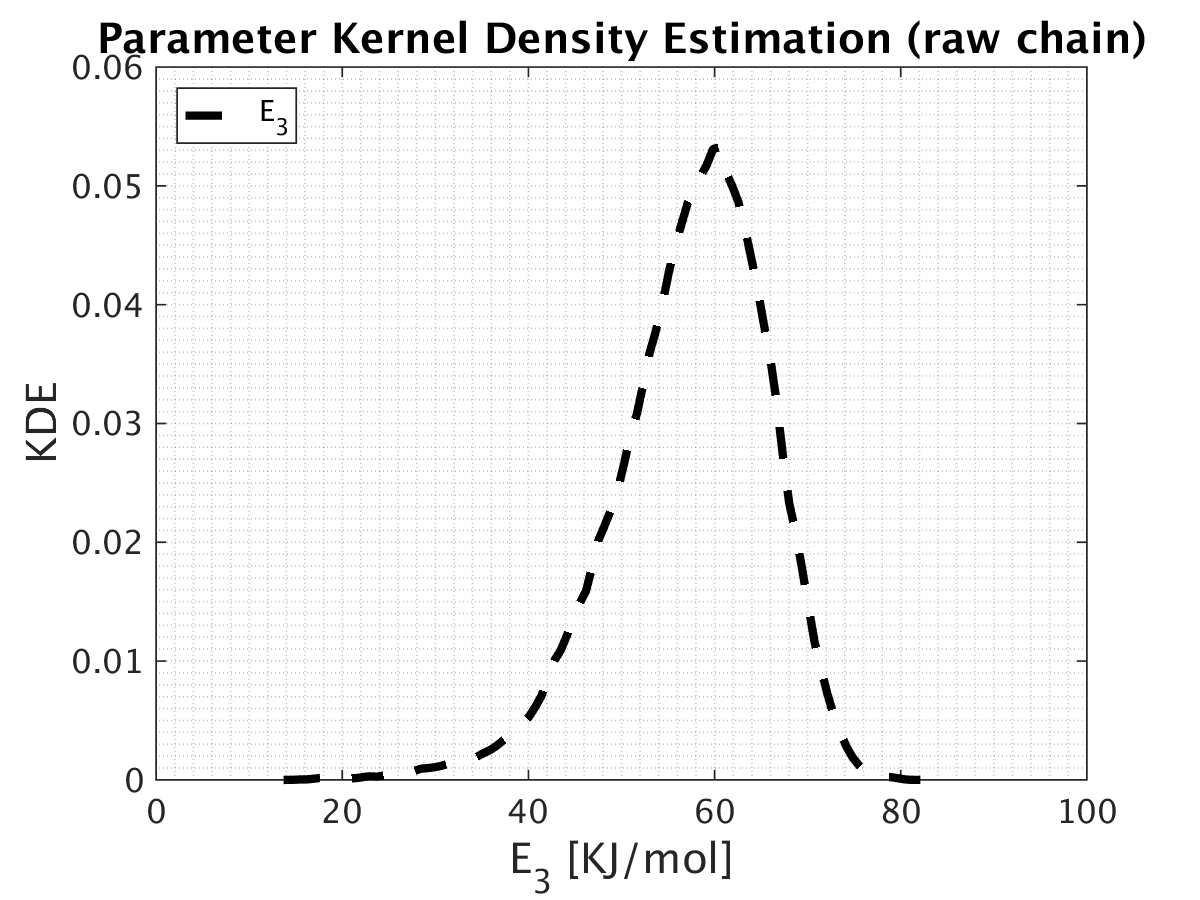
\includegraphics[scale=0.58]{model_3/kde_2} 
            }  
    \caption{Results for sample size 1e7}
\end{figure}

\begin{figure}[H]
\subfloat[log($A_3$) sample convergence \label{subfig-4:samp for $A_3$}]{
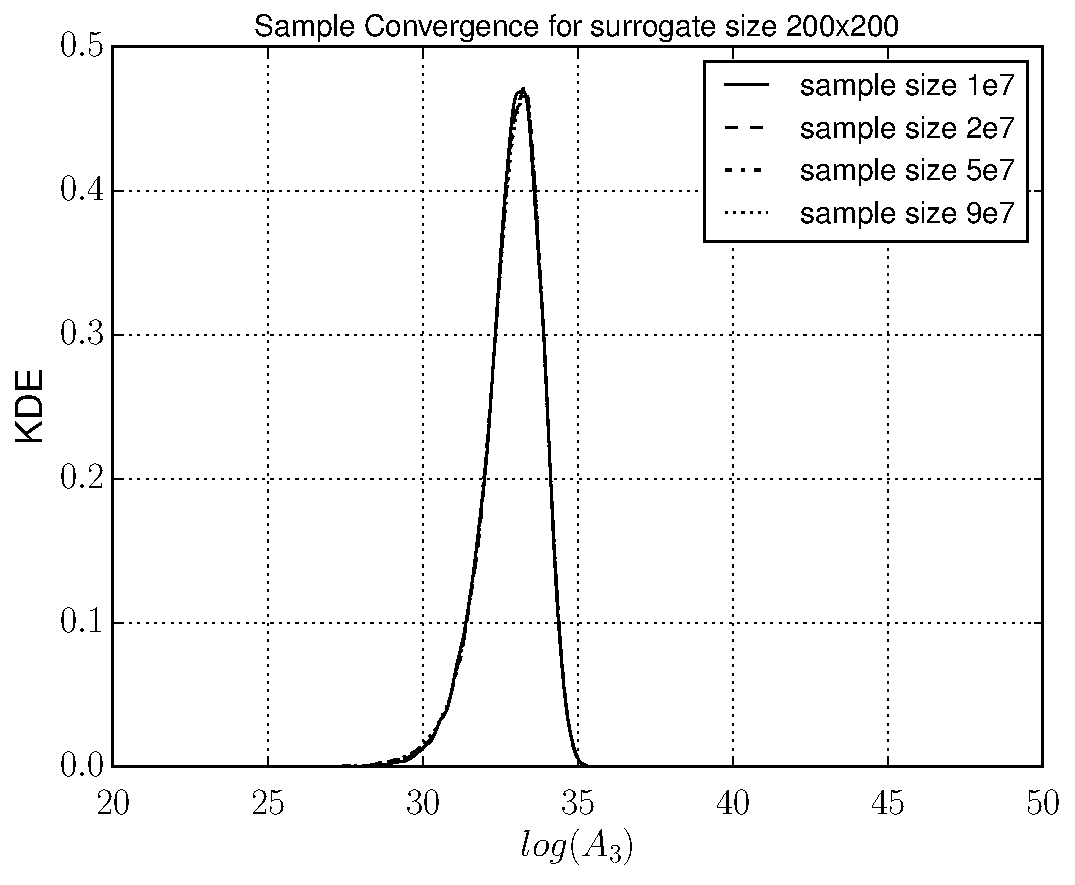
\includegraphics[scale = 0.45]{model_3/sample_conv_A3.pdf} 
				}
\subfloat[$E_3$ sample convergence \label{subfig-4:samp for $E_3$}]{
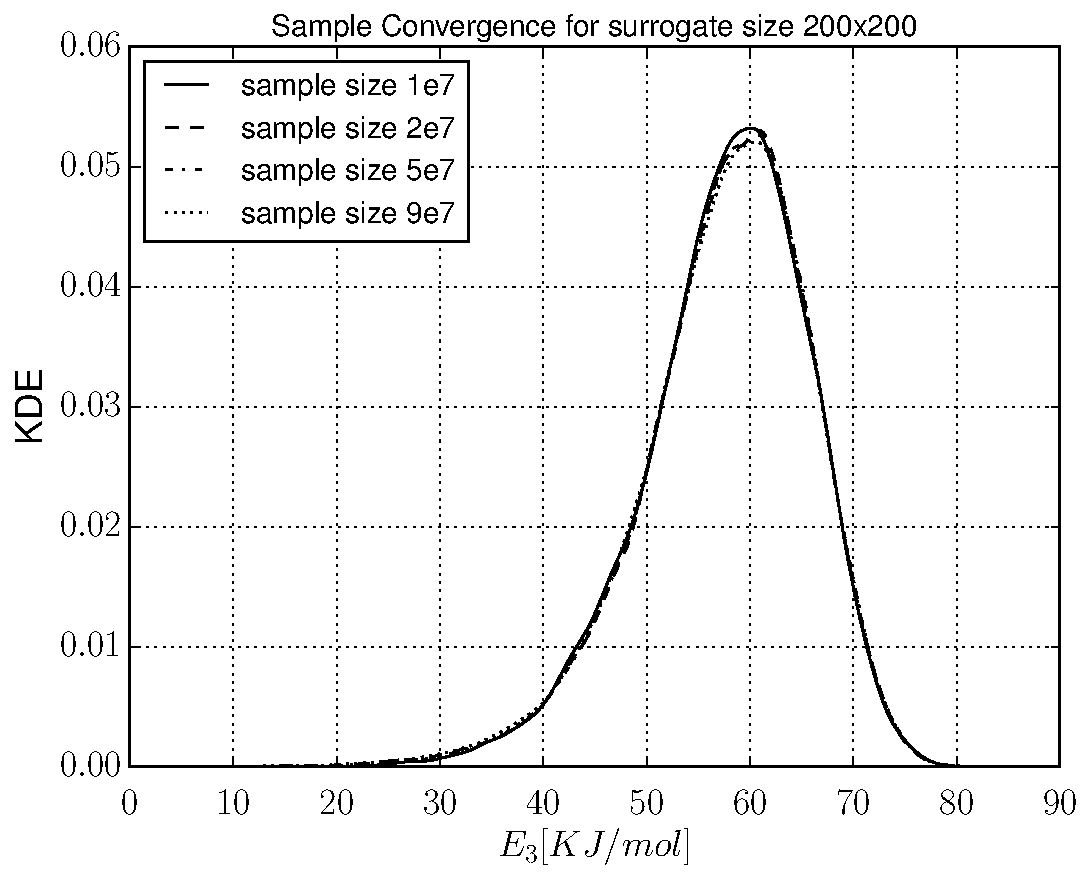
\includegraphics[scale = 0.45]{model_3/sample_conv_E3.pdf} 
				}
    \caption{Convergence for surrogate size 200x200}
\end{figure}

\begin{figure}[H]
\subfloat[log($A_3$) surrogate convergence \label{subfig-5:surr for $A_3$}]{
			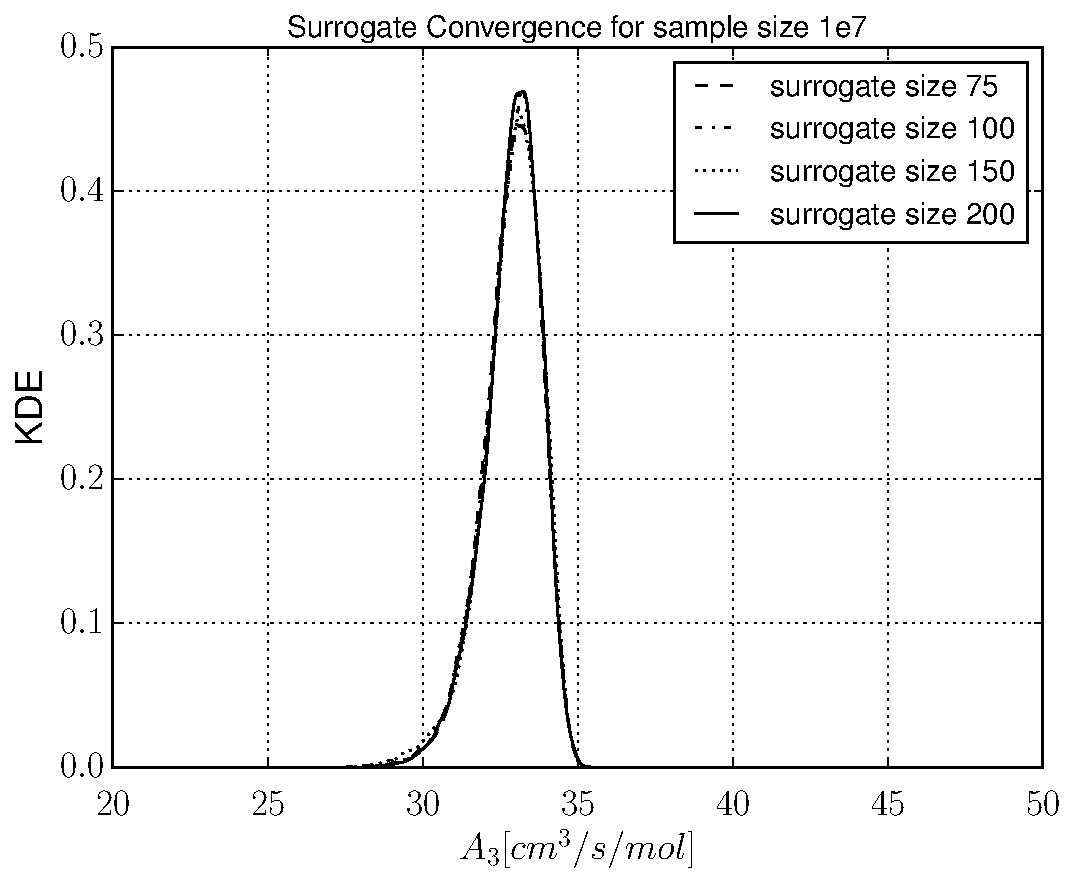
\includegraphics[scale = 0.45]{model_3/surrogate_conv_A3.pdf} 
				}
\subfloat[$E_3$ surrogate convergence \label{subfig-5:surr2 for $E_3$}]{
			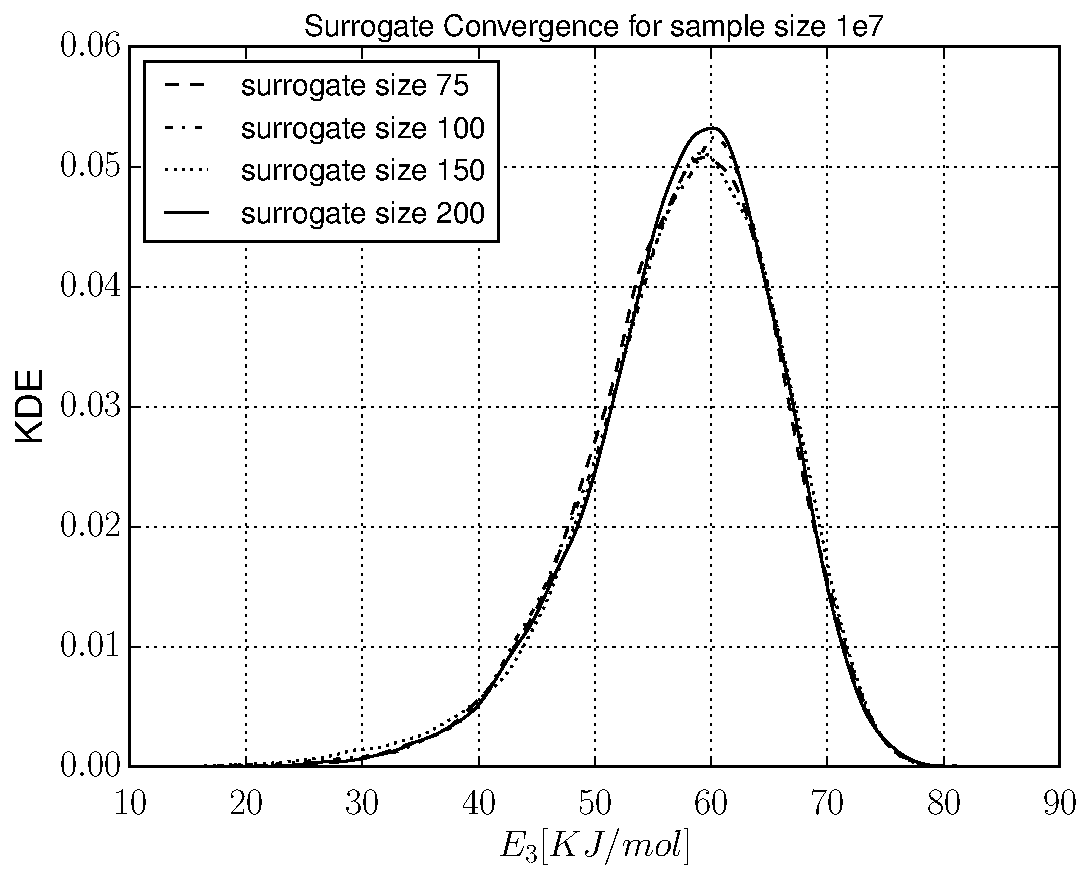
\includegraphics[scale = 0.45]{model_3/surrogate_conv_E3.pdf} 
				}
\caption{Convergence for sample size 1e7 with different number of surrogate points}
\end{figure}

 \begin{figure}[H]
   \subfloat[ Mean \label{subfig-1:mean_3}]{
        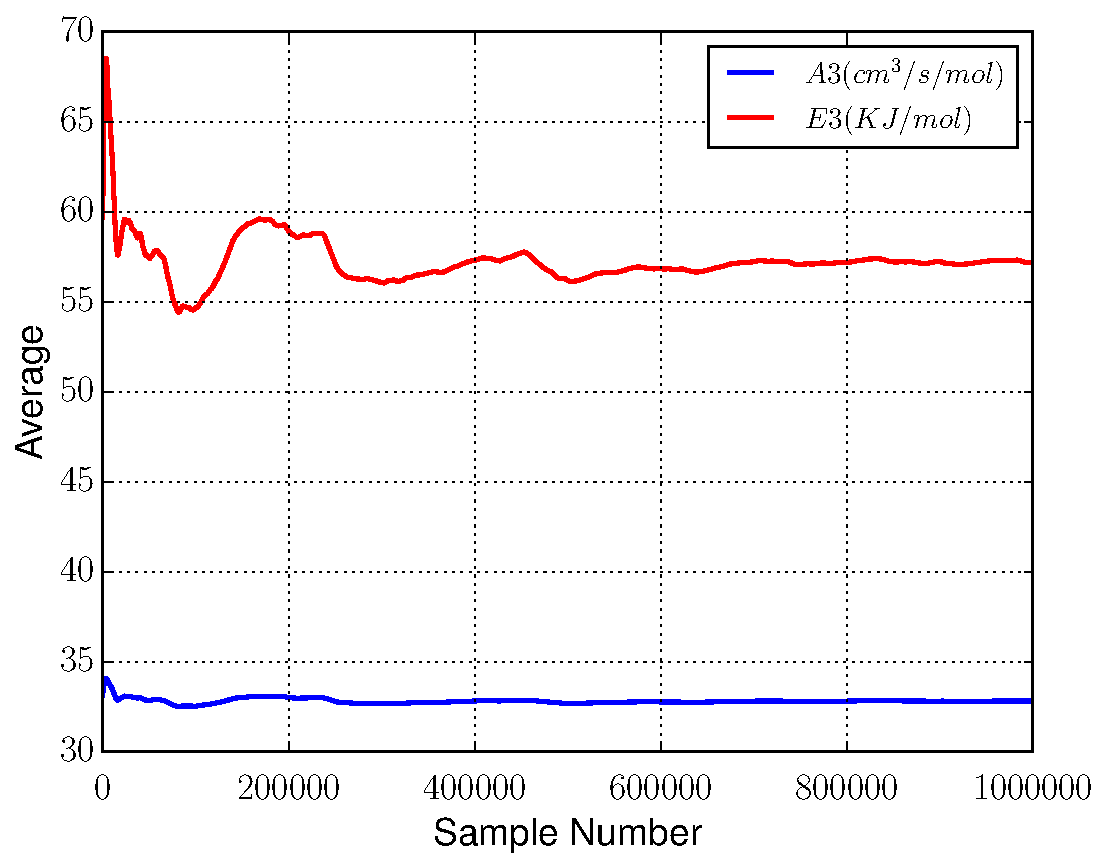
\includegraphics[scale=0.45]{model_3/M1_running_avg.pdf}
       }
\subfloat[Autocorrelation \label{subfig-2:autocr_3}]{
        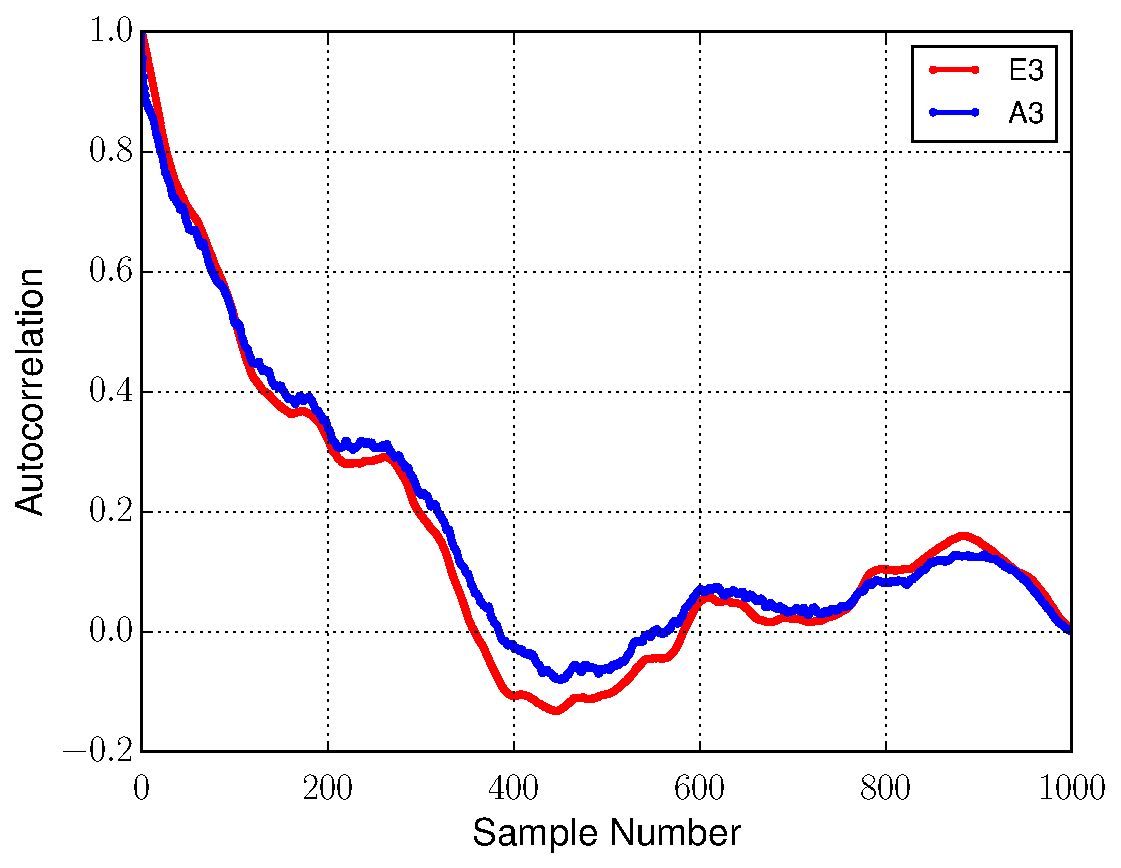
\includegraphics[scale=0.45]{model_3/M1_autocorr.pdf}
            }
            \caption{Mean and autocorrelation for sample size 1e6}
\end{figure}

 \begin{figure}[H]      
\subfloat[  $E_3$ distribution  \label{subfig-1:e3_distribution_3}]{
        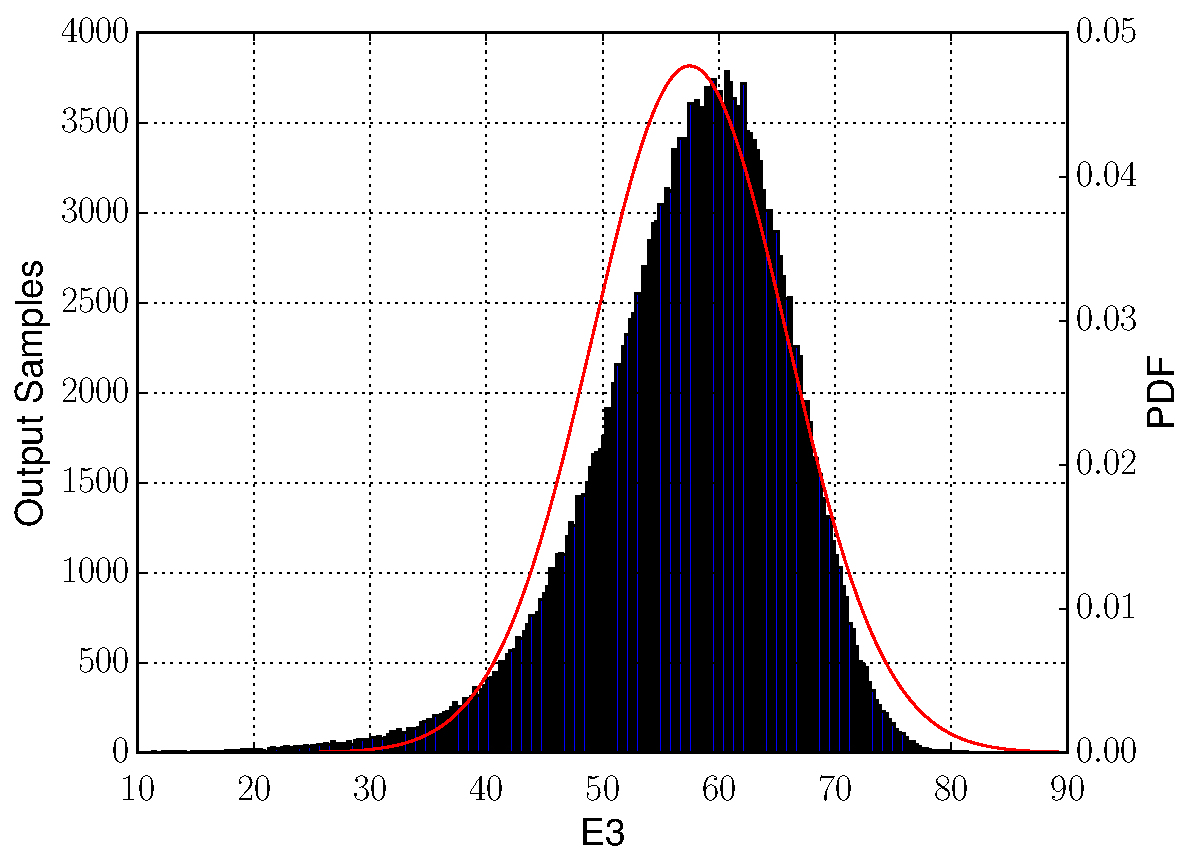
\includegraphics[scale=0.43]{model_3/E3.pdf} 
            }  
 \subfloat[ log($A_3$) distribution  \label{subfig-1:a3_distribution}]{
        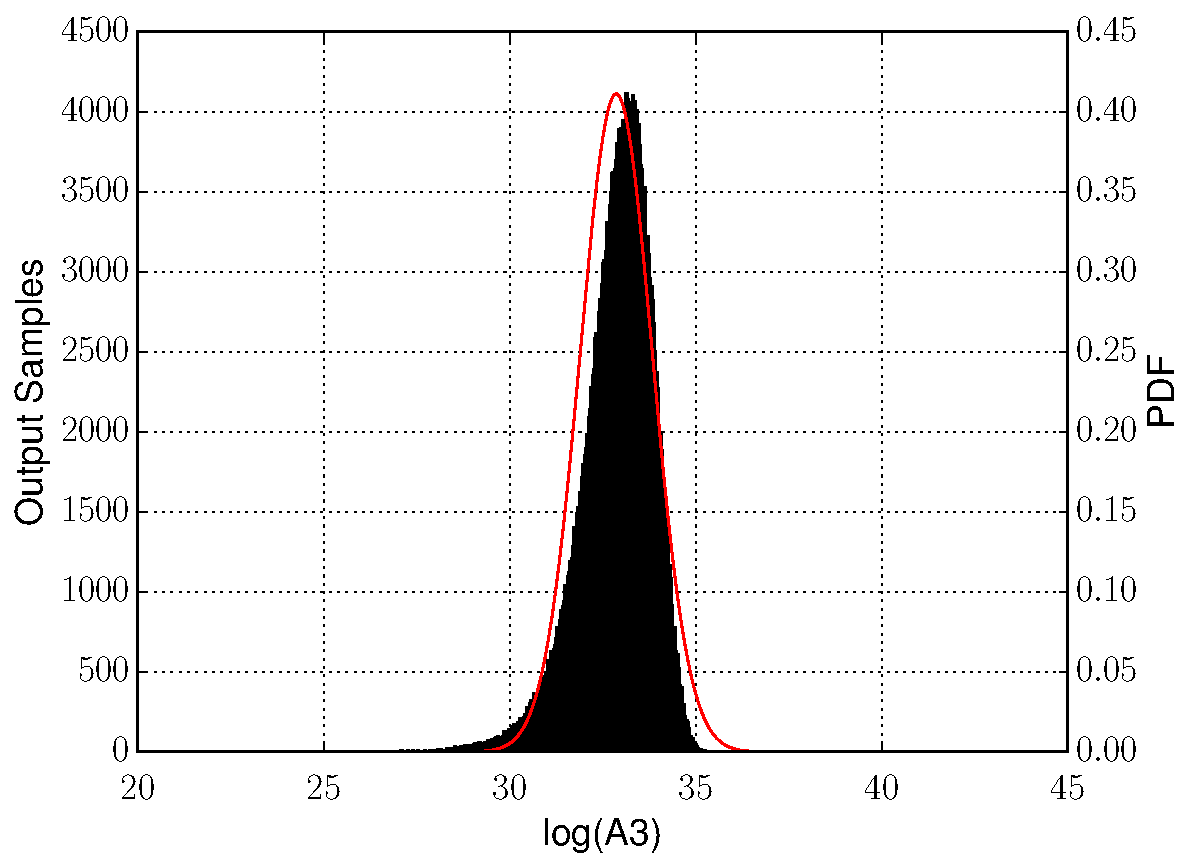
\includegraphics[scale=0.43]{model_3/A3.pdf}
            }
            \caption{$E_3$ and log($A_3$) posterior distributions}
\end{figure}

\subsection{Flamespeed Data Fit}

 It is necessary to ensure that the samples of the parameter which we are drawing are fitting the flamespeed values of the experiment. In this section, we calculate the flamespeed for all the parameters drawn using the surrogate generated before. We have taken $1e7$ sample size and calculated flamespeed for different concentrations of ozone. 

\begin{figure}[H]
   \subfloat[ Flame speed for 40 \% ozone \label{subfig-1:40_3}]{
        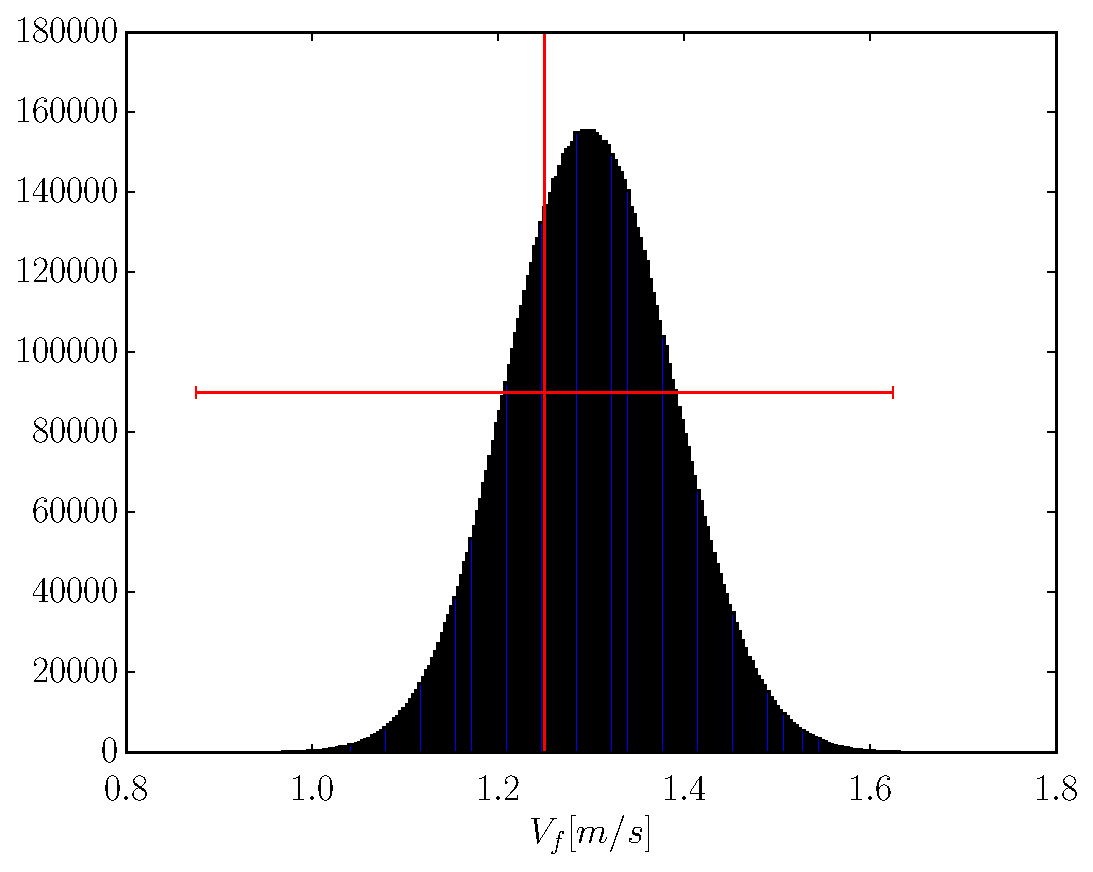
\includegraphics[scale=0.45]{model_3/flame_40.pdf}
       }
\subfloat[Flame speed for 46 \% ozone \label{subfig-2:46_3}]{
        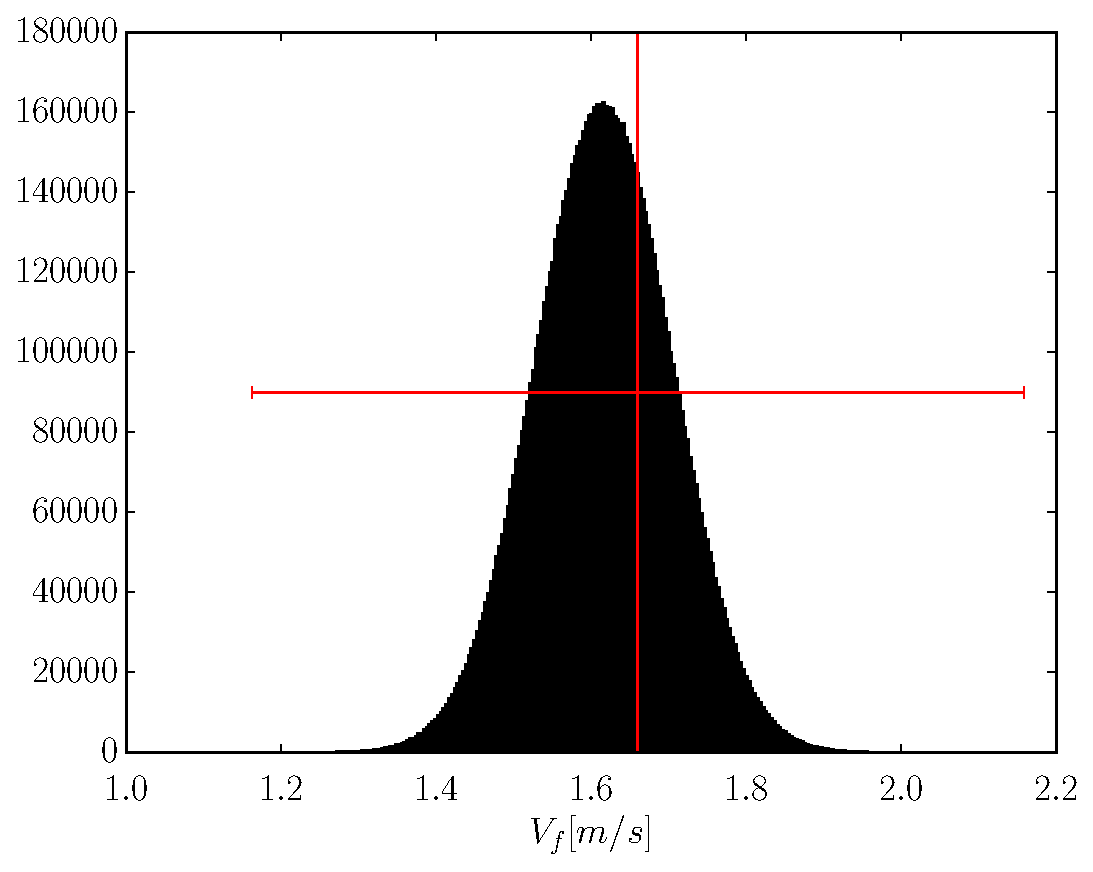
\includegraphics[scale=0.45]{model_3/flame_46.pdf}
            }
\end{figure}


 \begin{figure}[H]
  \ContinuedFloat
   \subfloat[ Flame speed for 53 \% ozone \label{subfig-3:53_3}]{
        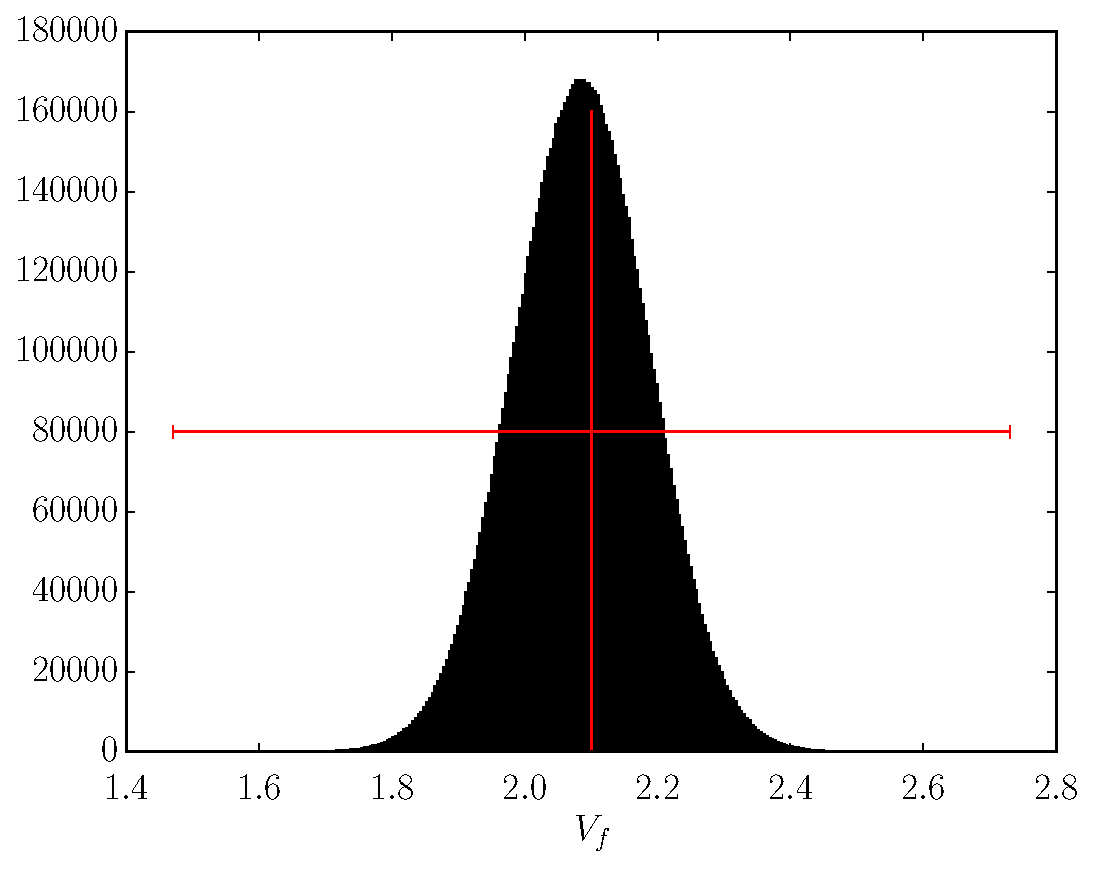
\includegraphics[scale=0.45]{model_3/flame_53.pdf}
       }
\subfloat[Flame speed for 75 \% ozone \label{subfig-4:75_3}]{
        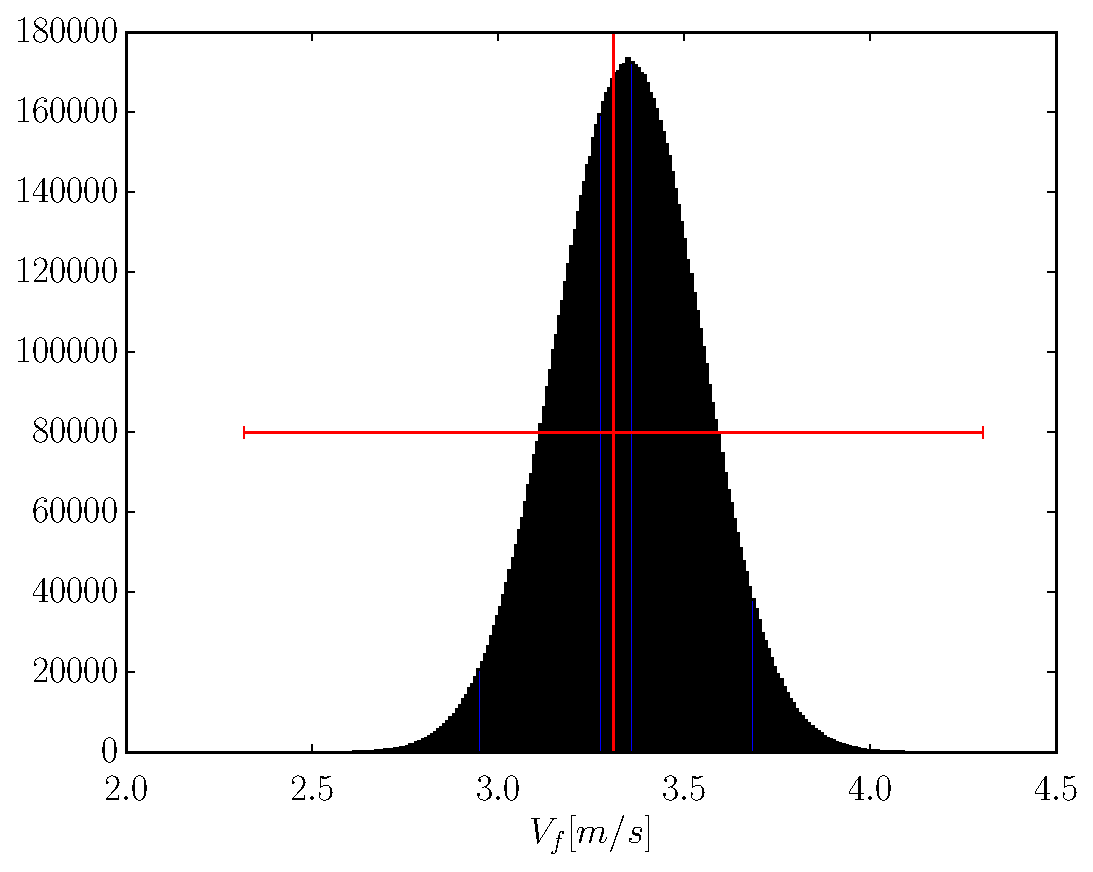
\includegraphics[scale=0.45]{model_3/flame_75.pdf}
            }
\end{figure}


 \begin{figure}[H]
  \ContinuedFloat
   \subfloat[ Flame speed for 100 \% ozone \label{subfig-5:100_3}]{
        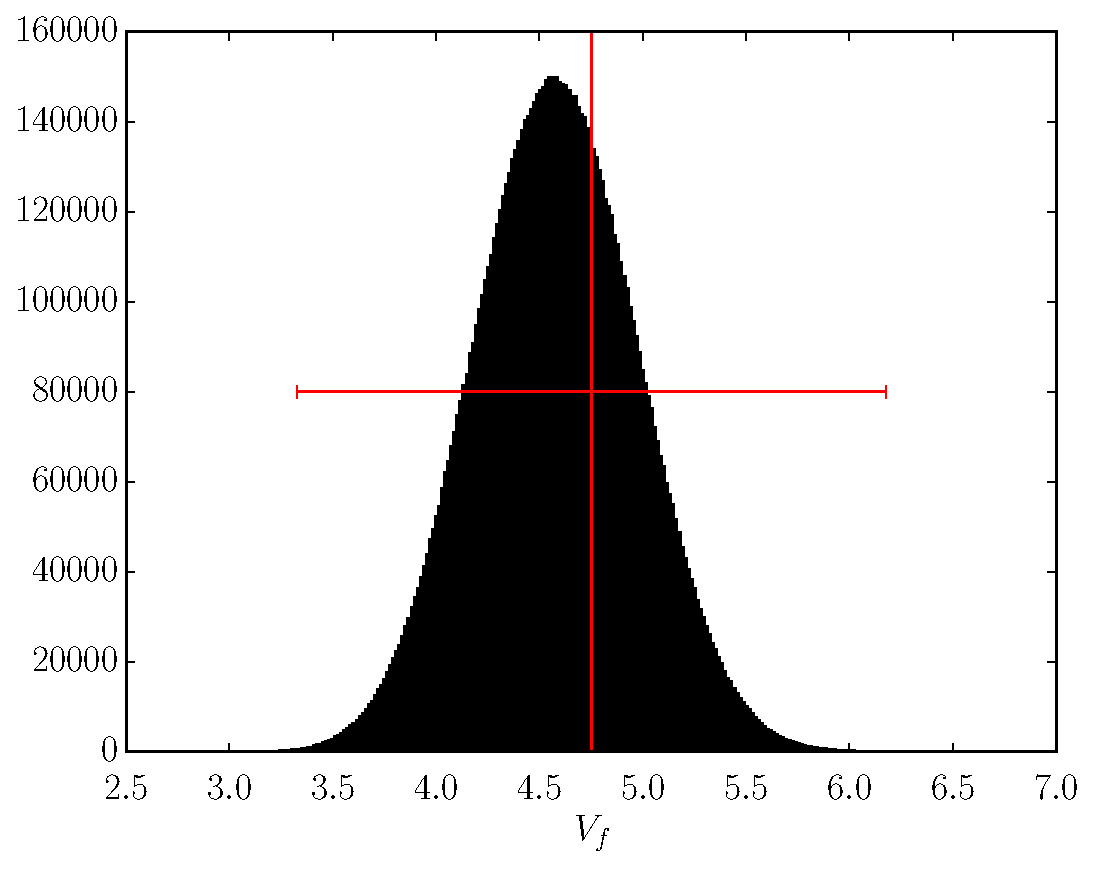
\includegraphics[scale=0.45]{model_3/flame_100.pdf}
       }
  \caption{Flamespeed data fit}
\end{figure}
